% =============================================
% Part 0.0 编辑个人信息
% =============================================

\newcommand{\department}{计算机学院}		%在这里修改系别
\newcommand{\major}{数据科学与大数据技术}				%在这里修改专业
\newcommand{\class}{大数据1701}					%在这里修改班级
\newcommand{\name}{	张丹颖		}			%在这里修改姓名
\newcommand{\stuid}{ 	2017011760	}				%在这里修改学号
\newcommand{\newdate}{	2018.10.07		}				%在这里修改日期 yyyy-mm-dd
\newcommand{\loc}{	学校	}					%在这里修改地点

% =============================================
% Part 0.1 编辑课程信息
% =============================================
\newcommand{\newcourse} {数据结构\LARGE{(C)}} %在这里修改成课程名称
\newcommand{\newtitle}{线性表的生成与操作} 				%在这里修改实验项目
\newcommand{\exptype}{计算机}

\newcommand{\grades}{}
\newcommand{\group}{无}

\newcommand{\tutor}{丁濛}
\newcommand{\onespace}{\hspace{1em} }
\begin{document}
\begin{titlepage}
	\centering
	\vspace*{1cm}
	{\fontsize{34pt}\baselineskip 实\onespace 验\onespace 报\onespace 告}\\
	\vspace{2cm}
	\fontsize{19pt}\baselineskip
	\makebox[30mm]{课程名称:}
	\underline{\makebox[75mm][c] {\newcourse} }
	\vskip 0.3cm
	\makebox[30mm]{实验项目:}
	\underline{\makebox[75mm][c] {\newtitle }}\\
	\vskip 0.3cm
	\makebox[30mm]{实验仪器:}
	\underline{\makebox[75mm][c]{计算机 }}\\%在这里修改实验仪器
	\vskip 1cm

    \begin{table}[!htbp]
      \centering
      \sihao
      \begin{tabular}{| c | c | c | c | c | c |}
      	\hline
        项目 & 报告格式 & 写作质量 & 逻辑、注释质量、思想描述 & 复杂度分析 & 合计\\
        \hline
        
        百分比(\%) & 15 & 25 & 40 & 20  & 100 \\
        \hline
        得分	& {\gradeFormat } & {\gradeCode } & {\gradeComment}   & {\gradeComplex} & {\gradeTotal} \\
        \hline
      \end{tabular}
    \end{table}
     \Comments
    	
	\vskip 2cm

        \begin{table}[!tbhp]
            \centering
            \sanhao
            \begin{tabular}{ll}
                系\hspace{2em}别:	&	 \underline {\makebox[60mm][c]	{\department} 	} \\
                专\hspace{2em}业:	&	 \underline {\makebox[60mm][c] {\major}		} \\
                班级姓名:		&	\underline {\makebox[60mm][c] {\class\ \name\ }		} \\
                日\hspace{2em}期:	&	 \underline {\makebox[60mm][c]	{\newdate} 	} \\
                成\hspace{2em}绩:	&	 \underline {\makebox[60mm][c] {\grades}		} \\
                同组成员:		&	\underline {\makebox[60mm][c] {\group}		} \\
                指导教师:		&	\underline {\makebox[60mm][c] {\tutor}		} \\
            \end{tabular}
        \end{table}


%    
%    

\end{titlepage}

\newpage
% =============================================
% Part 2 Main document
% =============================================
\xiaosihao
\section{实验目的}
\begin{enumerate}
\item 掌握线性表的顺序存储和链式存储结构;
\item 验证顺序表及链表的基本操作的实现;(验证)
\item 理解算法与程序的关系,能够将算法转换为对应程序;
\item 体会线性表在实际应用中能够解决的问题。(设计、综合)
\end{enumerate}

\section{实验内容}
\subsection{项目一}
实现顺序存储的线性表并分析每个功能的复杂度。要求具有如下功能:
\begin{enumerate}
\item 构造,析构;
\item 随机访问;
\item 在表后添加一个新数据;
\item 向表中特定位置插入一个新数据;
\item 将另外一张表内的内容添加到一个表的后面;
\item 查找表中是否含有特定元素;
\item 删除表中的某个特定元素;
\item 打印所有元素。
\end{enumerate}

\subsection{项目二}
实现链式存储的线性表(单向链表)并分析每个功能的复杂度。要求具有如下功能:
\begin{enumerate}
\item 构造,析构;
\item 在第一个元素之前插入一个新数据;在最后一个元素之后插入一个新数据;
\item 删除第一个元素;删除最后一个元素;
\item 查找表中是否含有特定元素; 
\item 向表中特定元素之前/之后插入一个新数据;
\item 删除表中的某个特定元素;
\item 遍历整个链表;
\item 反转一个链表,即 a->b->c->d, 反转后为 d->c->b->a.
\end{enumerate}

\subsection{项目三}
以双向链表的形式重新实现第2题,并分析两种实现中各个功能的复杂度区别。

\subsection{项目四}
完成上机平台上实验一的题目。

\section{实验过程}
\subsection{项目1}
大致思想:封装MyArray类,在主函数中实例化,实现其各种方法;
\begin{enumerate}
\item 构造和析构函数,令size=0和头指针置空(复杂度O(1));
\item 随机访问,直接利用数组下标访问(复杂度O(1));
\item 追加数字,由于数组容量有限,需要新开辟原size+1的空间,再把数字逐个复制过去(复杂度O(n));
\item 插入数字,开辟新空间,逐个将前index-1和后index+1复制,中间index位插入(复杂度O(n));
\item 追加表,开辟新空间,逐个将旧表和新表的值copy过去(复杂度O(n));
\item 查找特定元素,需要遍历(复杂度O(n));
\item 删除元素,从index位开始,后一位数覆盖前一位(复杂度O(n));
\item 打印,需要遍历(复杂度O(n))
\end{enumerate}

\subsubsection{实验步骤}
\subsubsection{必要代码}
\lstinputlisting[language=C++]{code/pro1_experiment1.cpp}
\subsubsection{实验结果}
	\begin{figure}[!bthp]
	\centering
        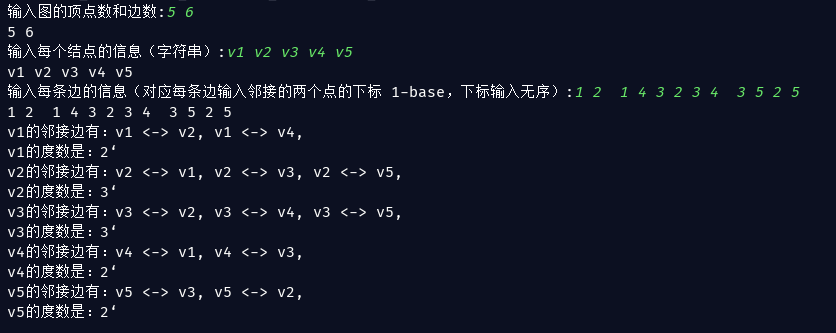
\includegraphics[width=0.6\linewidth]{1.PNG}
        \caption{问题一结果}
      \end{figure}

\subsection{项目2}
大致思想 :封装LinkList类,实现其各种方法
\begin{enumerate}
\item 构造和析构函数,为head结点开辟空间或释放空间(复杂度O(1));
\item 第一个元素之前插入(复杂度O(1));
\item 最后一个元素之后插入(复杂度O(1));
\item 删除第一个数(复杂度O(1));
\item 删除最后一个数(复杂度O(1));
\item 查找特定元素,需要遍历(复杂度O(n));
\item 元素之前插入,需要遍历找到该元素(复杂度O(n));
\item 元素之后插入,需要遍历(复杂度O(n));
\item 删除任意一个数,需要遍历(复杂度O(n));
\item 打印,需要遍历(复杂度O(n))
\item 递归反转,需要遍历找到倒数第二个结点(复杂度O(n))
\item 常规反转,需要遍历走一遍(复杂度O(n))
\end{enumerate}

\subsubsection{实验步骤}
\subsubsection{必要代码}
\lstinputlisting[language=C++]{code/pro2_experiment1.cpp}
\subsubsection{实验结果}
	\begin{figure}[!bthp]
	\centering
        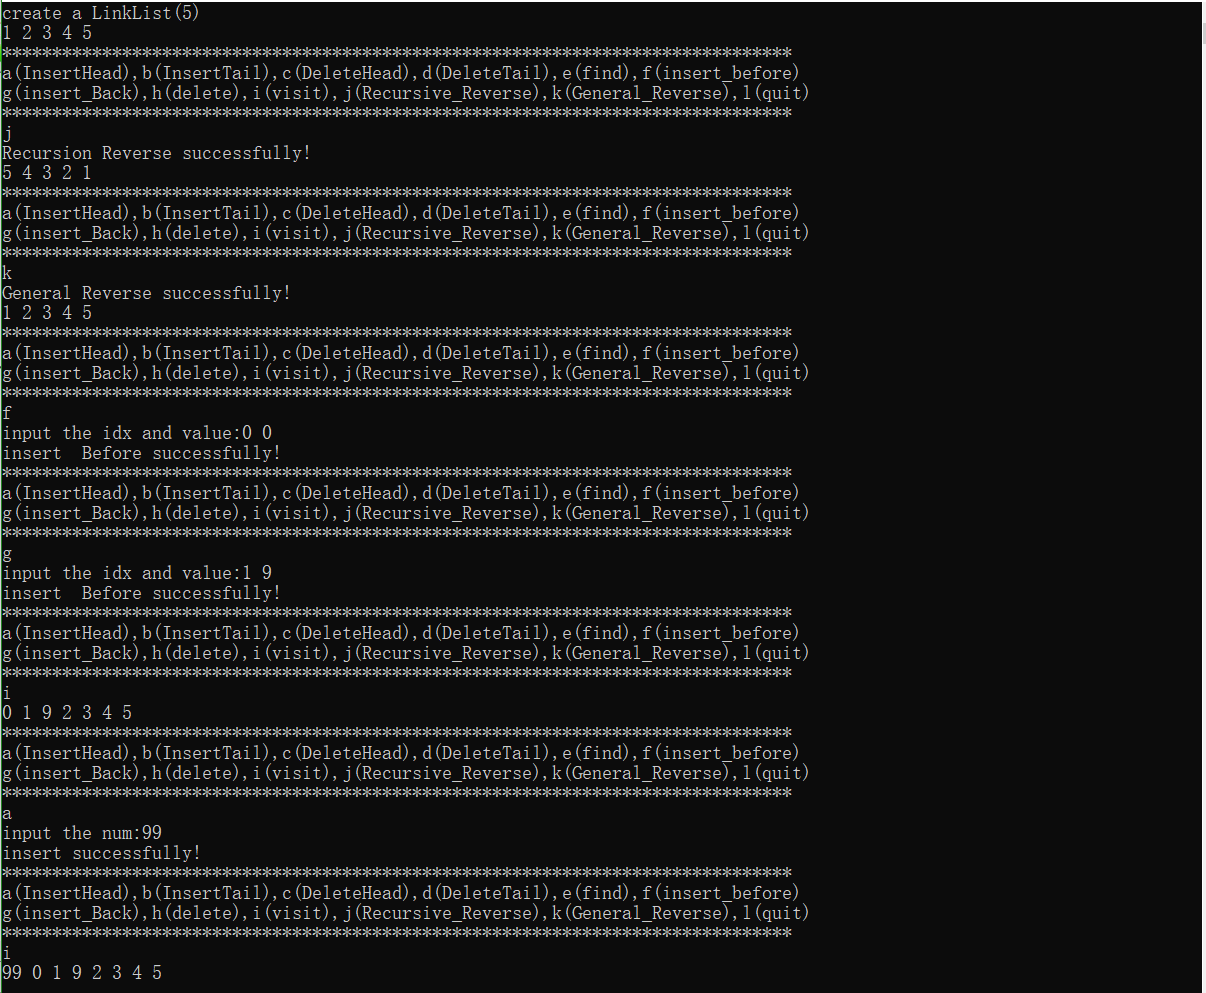
\includegraphics[width=0.6\linewidth]{2.PNG}
        \caption{问题二的结果}
      \end{figure}



\subsection{项目3}
大致思想 :除了反转以外,其他方法除了多处理一个pre指针以外,复杂度相同
\begin{enumerate}
\item 反转,也需要遍历走一遍(复杂度O(n)),但是只需要定义一个cur指针遍历,phead和ptial重点处理
\end{enumerate}
\subsubsection{实验步骤}
\subsubsection{必要代码}
\lstinputlisting[language=C++]{code/pro3_experiment1.cpp}
\subsubsection{实验结果}
	\begin{figure}[!bthp]
	\centering
        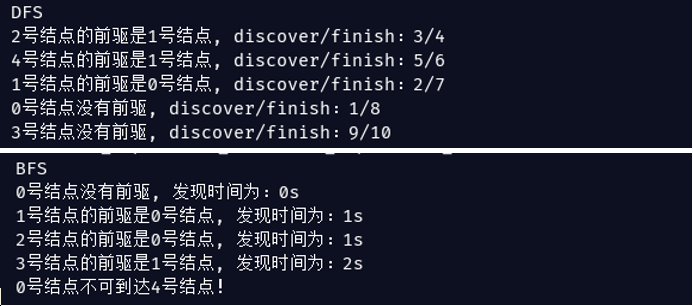
\includegraphics[width=0.6\linewidth]{3.PNG}
        \caption{问题三的结果}
      \end{figure}




\subsection{项目4.1}
大致思想 :TransStringToArray函数将String中的数字摘取存入数组中,Plus函数计算相加
\begin{enumerate}
\item TransStringToArray函数,用到while 循环,循环次数与字符串长度有关(复杂度O(n));
\item Plus函数,执行相加的次数,也与String长度相关(复杂度O(n))
\end{enumerate}
\subsubsection{实验步骤}
\subsubsection{必要代码}
\lstinputlisting[language=C++]{code/pro4.1_experiment1.cpp}
\subsubsection{实验结果}
	\begin{figure}[!bthp]
	\centering
        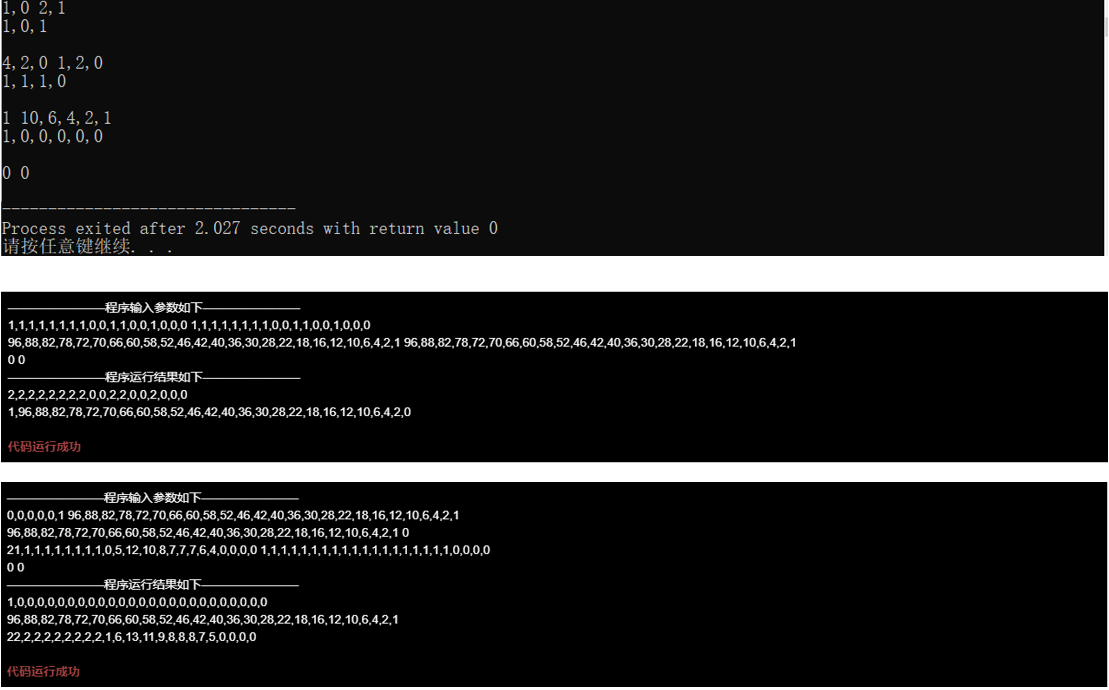
\includegraphics[width=0.6\linewidth]{4_1.PNG}
        \caption{问题4.1的结果}
      \end{figure}


\subsection{项目4.2}
大致思想 :对每个读入的成绩,在链表中,则该成绩出现次数++,否则,链表增加一个新结点
\begin{enumerate}
\item 复杂度(M*N),其中M代表要读入数字的规模,N代表已存在的链表结点规模(由于每次都要遍历,所以复杂度很高)
\end{enumerate}
\subsubsection{实验步骤}
\subsubsection{必要代码}
\lstinputlisting[language=C++]{code/pro4.2_experiment1.cpp}
\subsubsection{实验结果}
	\begin{figure}[!bthp]
	\centering
        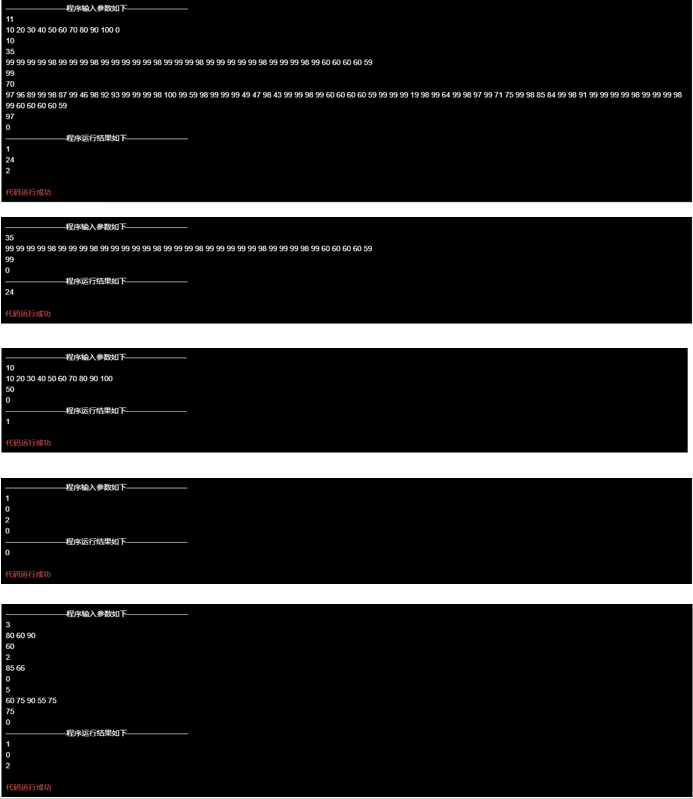
\includegraphics[width=0.6\linewidth]{4_2.PNG}
        \caption{问题4.2的结果}
      \end{figure}

\subsection{项目4.3}
大致思想 :plus函数中,首先去掉无效零,逐位将字符转换为数字再相加,满10进位,最后一次若要进位别忘了加上;
\begin{enumerate}
\item plus函数转换相加的复杂度取决于字符串长度(复杂度O(n));
\end{enumerate}
\subsubsection{实验步骤}
\subsubsection{必要代码}
\lstinputlisting[language=C++]{code/pro4.3_experiment1.cpp}
\subsubsection{实验结果}
		\begin{figure}[!bthp]
	\centering
        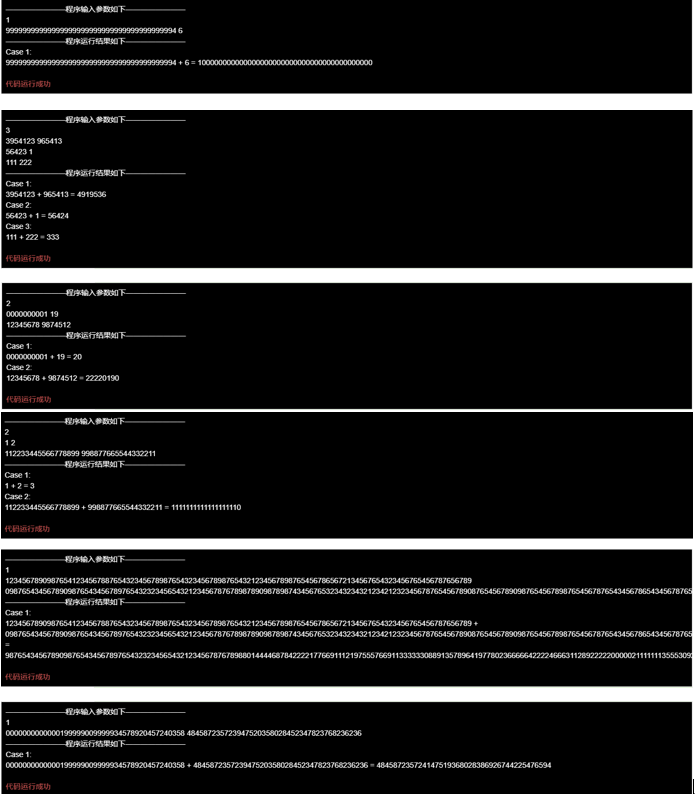
\includegraphics[width=0.6\linewidth]{4_3.PNG}
        \caption{问题4.3的结果}
      \end{figure}

\subsection{项目4.4}
大致思想 :Polynomial函数,对于系数数组每个数,都和其对应的x的几次方相乘,再相加,返回结果,不要用pow,可以直接利用上一次计算的结果;
\begin{enumerate}
\item (复杂度O(M*N)),N代表x最高项指数,M代表不同x的取值
\end{enumerate}
\subsubsection{实验步骤}
\subsubsection{必要代码}
\lstinputlisting[language=C++]{code/pro4.4_experiment1.cpp}
\subsubsection{实验结果}
	\begin{figure}[!bthp]
	\centering
        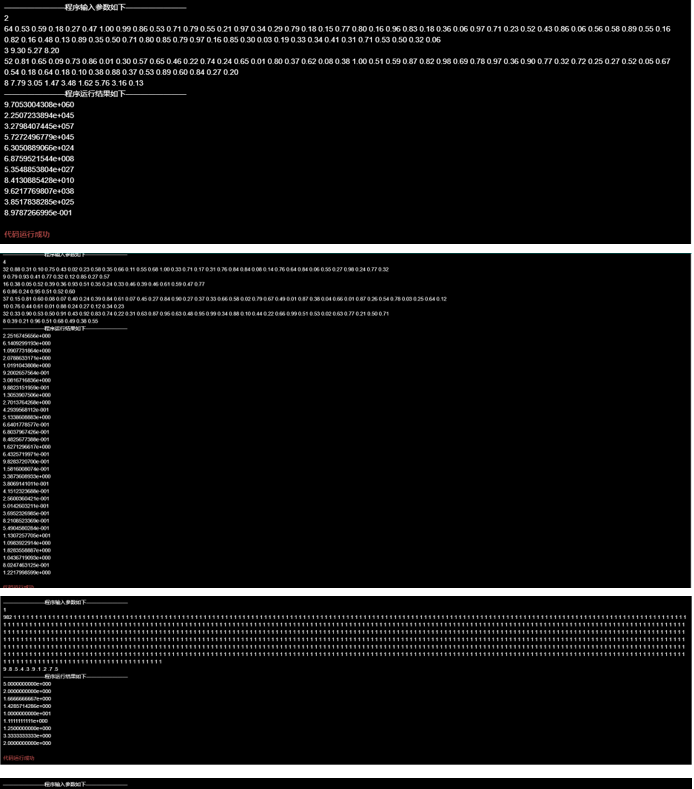
\includegraphics[width=0.6\linewidth]{4_4.PNG}
        \caption{问题4.4的结果}
      \end{figure}
\section{实验总结}
\subsection{优点}
\begin{enumerate}
\item 熟练掌握顺序存储和链式存储的线性表的增删改查等基本操作;
\item 掌握单链表和双向链表的反转,体会特殊结点特殊处理的思想;
\item  学会增加程序的鲁棒性;
\item  熟悉计算函数的复杂度;
\item  体会一个问题的多种解法,通过比较复杂度取优,以及用空间换时间;
\item  意识到线性表可以解决实际问题,如计算多项式,进位换算,查重;
\end{enumerate}
\subsection{不足}
\begin{enumerate}
\item 算法思想有待加强,逻辑思维能力不足,考虑问题不全面;
\end{enumerate}
\end{document}
